\documentclass[a4paper]{article}
\usepackage{fontspec}
\usepackage{amsmath}
\usepackage{amsfonts}
\usepackage{amssymb}
\usepackage{graphicx}
\usepackage{subcaption}
\usepackage[colorlinks=true,
linkcolor=blue,
citecolor=blue,
urlcolor=blue]
{hyperref}
\usepackage{cleveref}
\usepackage[left=1.00in, right=1.00in, top=1.00in, bottom=1.00in]{geometry}
\usepackage{lmodern}
\title{Introduction to Materials}
\author{Daniel Celis Garza}
\date{\today}
\begin{document}
\maketitle
	\section{Question 1}
	\subsection{a)}
	\subsubsection{i)}
		How many atoms in a BCC unit cell?
		
		\begin{figure}
			\centering
			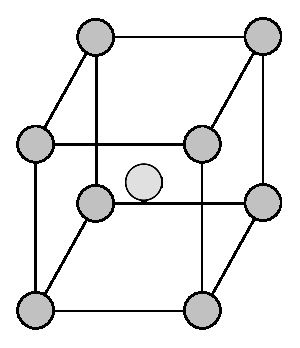
\includegraphics[width=0.33\linewidth]{bcc.eps}
			\caption{BCC unit cell.}
			\label{f:bcc}
		\end{figure}
		2 atoms per unit cell. $1/8$ atom per vertex, $1$ atom in the middle.
		
	\subsubsection{ii)}
		Estimate the density of Chromium (BCC) if the atomic radius, $R = 0.125$ nm, molar mass, $M = 52.0$ g/mol.
		
		\begin{figure}
			\centering
			\begin{subfigure}[b]{0.3\linewidth}
				\centering
				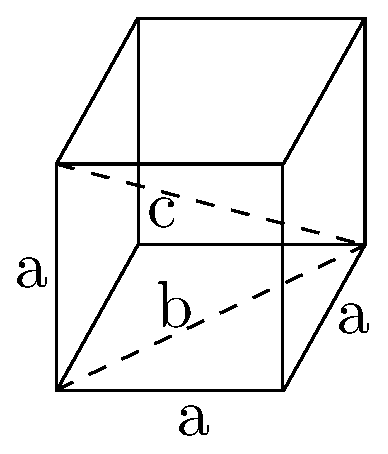
\includegraphics[width=\linewidth]{diag.eps}
				\caption{Cube diagonals.}
				\label{sf:diag}
			\end{subfigure}
			~
			\begin{subfigure}[b]{0.3\linewidth}
				\centering
				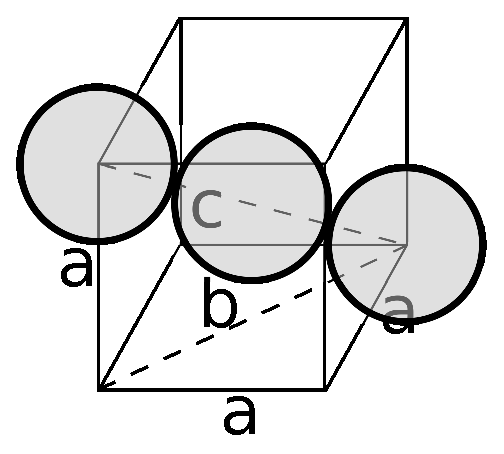
\includegraphics[width=\linewidth]{diag2.eps}
				\caption{Main diagonal (space filling).}
				\label{sf:diag2}
			\end{subfigure}
			~
			\begin{subfigure}[b]{0.3\linewidth}
				\centering
				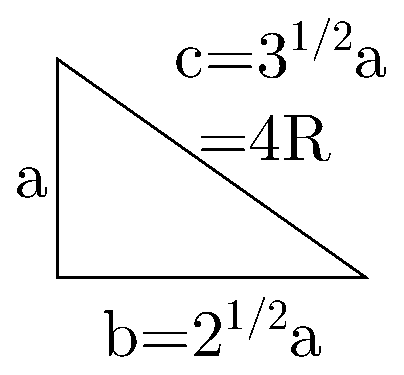
\includegraphics[width=\linewidth]{triag.eps}
				\caption{Diagonal values.}
				\label{sf:diag3}
			\end{subfigure}
			\label{f:diag}
		\end{figure}
		Density,
		\begin{align}
			\rho = m/v~, \label{e:dens}
		\end{align}
		where $m \equiv $ mass and $v \equiv $ volume. From \cref{f:diag} we find,
		\begin{align}
			a &= \dfrac{4}{\sqrt{3}} R \\
			v_{\textrm{unit cell}} &= a^{3} = \left(\dfrac{4}{\sqrt{3}}\right)^{3} R^{3}~, \label{e:volume}
		\end{align}
		The mass of a BCC metal in a unit cell, 
		\begin{align}
			m_{\textrm{unit cell}} = M \times \dfrac{2}{A_{N}}, \label{e:mass}
		\end{align} 
		where $2 \equiv $ number of atoms in a unit cell and $A_{N} \equiv $ avogadro's constant. Substituting \cref{e:volume, e:mass} into \cref{e:dens} we obtain an expression for the density of any BCC metal using values for its unit cell,
		\begin{align}
			\rho = \dfrac{2 \sqrt{3^{3}} M }{4^{3} R^{3} A_{N}}~.
		\end{align}
		Substituting the relevant values we find \cref{se:rho},
		\begin{subequations}
		\begin{align}
			\rho &= \dfrac{2 \sqrt{27} \times 52.0}{4^{3} \left(0.125 \times 10^{-7} \right)^{3} 6.022 \times 10^{23} \textrm{atom/mol}} \dfrac{[\textrm{atom g mol$^{-1}$}]}{[\textrm{atom cm$^{3}$ mol$^{-1}$}]}\\
			\rho &= 7.18 \textrm{ g/cm$^{3}$} \label{se:rho}\\
			\rho_{\textrm{real}} &= 7.15 \textrm{ g/cm$^{3}$}~.
		\end{align}
		\end{subequations}
		
		\subsection{b)}
		\subsubsection{i)}
		\begin{align}
			v_{1} &= \begin{bmatrix}
					1 & 2 & 3
					\end{bmatrix}\\
			v_{2} &= \begin{bmatrix}
					1 & 1 & -1
					\end{bmatrix}\\
			v_{3} &= \begin{bmatrix}
					1 & 1 & 1
					\end{bmatrix}~.
		\end{align}
		Show $v_{1} \parallel v_{2}$ and not to $v_{3}$.
		
		By the dot product,
		\begin{subequations}		
		\begin{align}
			v_{1} \cdot v_{2} &= \begin{bmatrix}
								1 & 2 & 3
								\end{bmatrix} 
								\begin{bmatrix}
								1\\
								1\\
								-1
								\end{bmatrix}
							    = 1 + 2 - 3 = 0\\
			v_{1} \cdot v_{3} &= \begin{bmatrix}
								1 & 2 & 3
								\end{bmatrix} 
								\begin{bmatrix}
								1\\
								1\\
								1
								\end{bmatrix}
								= 1 + 2 + 3 = 6~.
		\end{align}
		\end{subequations}
	\subsubsection{ii)}
	The zone axis refers to translational invariance between planes. They're described as integer basis vectors such that translations by the basis vector can move any plane to another with the same zone axis. Essentially they are a linear map $f: R^{2} \to R^{2'}$, $f$ being the zone axis. Represented here as the trace of a $3\times3$ matrix.
	\begin{align}
		\begin{bmatrix}
		u & v & w
		\end{bmatrix} &\to 
		\begin{bmatrix}
		u' & v' & w'
		\end{bmatrix}\\
		\begin{bmatrix}
		u & v & w
		\end{bmatrix}
		\begin{bmatrix}
		a & 0 & 0\\
		0 & b & 0 \\
		0 & 0 & c
		\end{bmatrix}
		&=
		\begin{bmatrix}
		u' & v' & w'
		\end{bmatrix}~.
	\end{align}
	\subsubsection{iii)}
	The indices of zone axis can be found by simple vector subtraction of the parallel plane, and multiplying by the smallest factor so all numbers are integer values.
	\begin{align}
		v_{1} - v_{2} = 
		\begin{bmatrix}
		0 & 1 & 4
		\end{bmatrix}~.
	\end{align}
	
	\subsection{c)}
	Cu$_{3}$Au has an FCC lattice. If the collection of atoms is translated to all vertices of the unit cell we obtain an FCC lattice.
	\begin{figure}
		\centering
		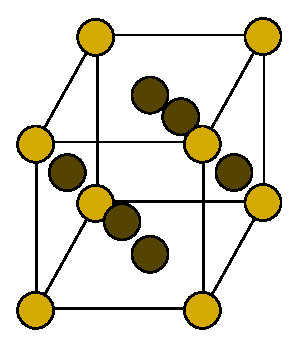
\includegraphics[width=0.33\linewidth]{cu3au.eps}
		\caption{Cu$_{3}$Au unit cell.}
	\end{figure}
\end{document}